\chapter{Arquitetura e Modelagem do Sistema} \label{cha:arquitetura}

\section{Arquitetura da Solução}
Esta seção descreve a organização estrutural do sistema ViaBus, que provê funções de gestão de transporte para empresas: cadastro de empresas, usuários, motoristas, veículos, rotas, paradas, viagens e bilhetes. A solução adota uma arquitetura web em camadas, com separação clara entre apresentação (frontend), lógica de negócio e APIs (backend) e persistência (banco de dados).

No \textit{frontend}, utiliza-se Next.js~15 com roteamento via App Router, estado de sessão via NextAuth (estratégia \textit{JWT}) e componentes React tipados (TypeScript). O \textit{frontend} consome APIs REST autenticadas, mantém contexto de usuário/empresa e incorpora mapas e edição geográfica com Leaflet/React-Leaflet para operações sobre rotas e paradas.

O \textit{backend} é implementado com NestJS~11, estruturado por módulos de domínio (\textit{auth}, \textit{users}, \textit{companies}, \textit{drivers}, \textit{vehicles}, \textit{stops}, \textit{routes}, \textit{trips}, \textit{tickets}, etc.). As regras de negócio são expostas por controladores REST, protegidos por autenticação \textit{JWT} e autorização baseada em papéis. A multiempresa é tratada por \textit{companyId} e por um interceptor que injeta o contexto de empresa a partir do token. A persistência usa TypeORM com PostgreSQL.

\begin{figure}[H]
  \centering
  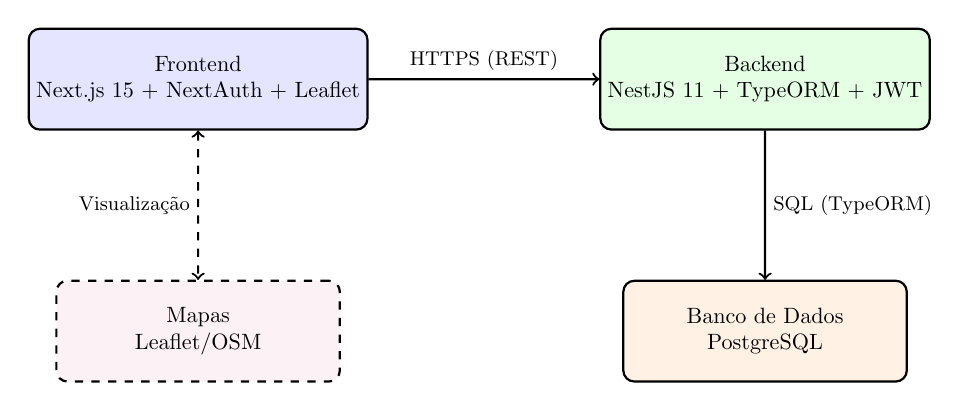
\begin{tikzpicture}[scale=0.8, every node/.style={transform shape}]
    \tikzumlset{font=\footnotesize}
    % Blocos
    \node[draw, rounded corners, thick, fill=blue!10, minimum width=4.5cm, minimum height=1.6cm, align=center] (fe) at (0,2) {\text{Frontend}\\Next.js 15 + NextAuth + Leaflet};
    \node[draw, rounded corners, thick, fill=green!10, minimum width=4.5cm, minimum height=1.6cm, align=center] (be) at (9,2) {\text{Backend}\\NestJS 11 + TypeORM + JWT};
    \node[draw, rounded corners, thick, fill=orange!10, minimum width=4.5cm, minimum height=1.6cm, align=center] (db) at (9,-2) {\text{Banco de Dados}\\PostgreSQL};
    \node[draw, dashed, rounded corners, thick, fill=purple!5, minimum width=4.5cm, minimum height=1.6cm, align=center] (maps) at (0,-2) {\text{Mapas}\\Leaflet/OSM};

    % Conexões
    \draw[->, thick] (fe) -- node[above, font=\small]{HTTPS (REST)} (be);
    \draw[->, thick] (be) -- node[right, font=\small]{SQL (TypeORM)} (db);
    \draw[<->, thick, dashed] (fe) -- node[left, font=\small]{Visualização} (maps);
  \end{tikzpicture}
  \caption{Visão de alto nível da solução.}
\end{figure}

\section{Modelagem do Banco de Dados}

O modelo de dados foi projetado para refletir as agregações de negócio, garantindo a coesão e a integridade das entidades do domínio. A \autoref{tab:principais-entidades} sumariza as principais entidades e seus papéis. Para facilitar a análise, a modelagem será apresentada através de diagramas UML fracionados por agregado. A visão completa e detalhada de todos os relacionamentos do domínio está disponível para consulta no \autoref{apendice:diagrama-classe}.

\begin{table}[H]
  \small
  \centering
  \begin{tabular}{p{3.5cm}p{11.5cm}}
    \toprule
    \text{Entidade}           & \text{Descrição resumida}                                                                                                                                                \\
    \midrule
    \texttt{companies}        & Empresa (razão social, nome fantasia, CNPJ, slug, e-mail, telefone, logo)                                                                                                \\
    \texttt{users}            & Usuário (nome, e-mail, senha, papel, status, telefone, foto, \texttt{company\_id})                                                                                       \\
    \texttt{drivers}          & Motorista (nome, CPF, CNH, categoria, validade, telefone, e-mail, data nascimento, contratação, status, contato emergência, endereço, observações, \texttt{company\_id}) \\
    \texttt{vehicles}         & Veículo (placa, modelo, marca, ano, capacidade, categoria, conforto, tipo ônibus, data aquisição, hodômetro, manutenção, status, observações, \texttt{company\_id})      \\
    \texttt{addresses}        & Endereço (CEP, logradouro, número, complemento, bairro, cidade, estado, longitude, latitude)                                                                             \\
    \texttt{stops}            & Parada (nome, \texttt{address\_id}, ativa, acessibilidade, abrigo, \texttt{company\_id})                                                                                 \\
    \texttt{routes}           & Rota (nome, descrição, ativa, duração estimada, distância, \texttt{company\_id})                                                                                         \\
    \texttt{route\_stops}     & Associação rota–parada com ordem e horário de partida opcional                                                                                                           \\
    \texttt{route\_schedules} & Agenda por dia da semana para a rota (0-6, domingo-sábado)                                                                                                               \\
    \texttt{trips}            & Viagem (rota, horários partida/chegada, status, preço base, assentos total/disponível, auto-gerada, observações, \texttt{company\_id})                                   \\
    \texttt{trip\_vehicles}   & Associação viagem–veículo com motoristas primário/secundário                                                                                                             \\
    \texttt{tickets}          & Bilhete (passageiro, documento, telefone, e-mail, assento, preço, status, pontos embarque/desembarque com coordenadas, observações, \texttt{company\_id})                \\
    \bottomrule
  \end{tabular}
  \caption{Principais entidades do domínio.}
  \label{tab:principais-entidades}
\end{table}

\subsection{Diagramas UML Fracionados por Agregado}

Para facilitar a análise do domínio e a compreensão das decisões de modelagem, o esquema de dados foi decomposto em agregados lógicos. Um agregado é um cluster de objetos de domínio que podem ser tratados como uma única unidade, garantindo a consistência das regras de negócio. A seguir, cada agregado principal é detalhado, justificando-se as principais decisões de modelagem.

\subsubsection*{Agregado Organizacional: Empresas e Usuários}

O pilar da arquitetura multi-tenant do sistema reside neste agregado. A entidade \texttt{Company} é a raiz de todos os dados operacionais. A decisão de incluir a chave estrangeira \texttt{companyId} na entidade \texttt{User} estabelece o vínculo fundamental que garante que cada usuário pertença inequivocamente a uma única empresa. Este design é a base para o filtro de isolamento de dados que será aplicado em todas as consultas subsequentes, conforme detalhado na seção de arquitetura do backend.

\begin{figure}[H]
  \centering
  \begin{tikzpicture}[scale=0.8, every node/.style={transform shape}]
    \tikzumlset{font=\footnotesize}

    \umlclass[x=0,y=0]{Company}{
      id: uuid\\
      legalName: string\\
      tradeName: string\\
      slug: string\\
      cnpj: string\\
      email: string\\
      phone: string\\
      logoUrl: string
    }{ }

    \umlclass[x=8,y=0]{User}{
      id: uuid\\
      name: string\\
      email: string\\
      phone: string\\
      photoUrl: string\\
      password: string\\
      role: UserRole\\
      status: UserStatus\\
      companyId: uuid
    }{ }

    % --- ALTERAÇÃO PRINCIPAL AQUI ---
    % Trocamos \umlassoc por \umluniaggreg para criar o losango de agregação
    \umluniaggreg[mult1=1,mult2=*]{Company}{User}

    \umlnote[x=0,y=-4, width=12cm]{Company}{Escopo multiempresa: todas as entidades operacionais possuem \texttt{companyId} para isolamento de dados}
  \end{tikzpicture}
  \caption{Agregado organizacional - estrutura multiempresa.}
\end{figure}

\subsubsection*{Agregado de Configuração: Rotas e Paradas}

Este agregado modela a estrutura logística fundamental de uma empresa de transporte. A decisão mais crítica aqui foi a criação da entidade associativa \texttt{RouteStop}. Em vez de uma relação simples, a \texttt{RouteStop} foi necessária para resolver o relacionamento N:N entre \texttt{Route} e \texttt{Stop}, permitindo que uma mesma parada (ex: "Rodoviária de Picos") possa pertencer a múltiplas rotas. Mais importante, esta entidade armazena o atributo \texttt{order}, que é a regra de negócio central para definir a sequência do trajeto, transformando um conjunto de pontos em um itinerário ordenado. Adicionalmente, a entidade \texttt{RouteSchedule} foi criada para desacoplar a definição da rota de sua frequência operacional, permitindo que uma mesma rota tenha horários diferentes dependendo do dia da semana.

\begin{figure}[H]
  \centering
  \begin{tikzpicture}[scale=0.7, every node/.style={transform shape}]
    % Aumentando a fonte para melhor legibilidade
    \tikzumlset{font=\footnotesize}

    % Entidades reorganizadas para melhor fluxo visual
    \umlclass[x=6,y=7]{Route}{
      id: uuid\\
      name: string\\
      description: string\\
      isActive: boolean\\
      estimatedDuration: string\\
      distance: number\\
      companyId: uuid
    }{ }

    \umlclass[x=0,y=2]{RouteSchedule}{
      id: uuid\\
      routeId: uuid\\
      dayOfWeek: number\\
      isActive: boolean\\
      createdAt: Date\\
      updatedAt: Date
    }{ }

    \umlclass[x=6,y=2]{RouteStop}{
      id: uuid\\
      routeId: uuid\\
      stopId: uuid\\
      order: number\\
      departureTime: string
    }{ }

    \umlclass[x=12,y=2]{Stop}{
      id: uuid\\
      name: string\\
      addressId: uuid\\
      isActive: boolean\\
      hasAccessibility: boolean\\
      hasShelter: boolean\\
      companyId: uuid
    }{ }

    \umlclass[x=17,y=2]{Address}{
      id: uuid\\
      cep: string\\
      street: string\\
      ...
    }{ }

    % --- RELACIONAMENTOS ESPECÍFICOS ---
    % Composição: Route "possui" seus RouteSchedules. Se a rota for apagada, seus horários também são.
    \umlcompo[mult1=1, mult2=*]{Route}{RouteSchedule}

    % Composição: Route "possui" sua sequência de paradas (RouteStop).
    \umlcompo[mult1=1, mult2=*]{Route}{RouteStop}

    % Associação: RouteStop "aponta para" uma Stop. A Stop existe independentemente.
    \umluniassoc[mult1=*, mult2=1]{RouteStop}{Stop}

    % Composição: Stop "possui" um Address.
    \umlcompo[mult1=1, mult2=1]{Stop}{Address}

    \umlnote[x=4,y=-2, width=10cm]{RouteStop}{
      \texttt{RouteStop} é uma classe associativa que resolve o relacionamento N:N entre \texttt{Route} e \texttt{Stop}, adicionando o atributo de ordem (\texttt{order}).
    }
  \end{tikzpicture}
  \caption{Agregado de configuração de rotas, paradas e horários.}
\end{figure}

\subsubsection*{Agregado de Recursos Operacionais: Veículos e Motoristas}

Este agregado representa os ativos físicos e humanos da empresa. As entidades \texttt{Vehicle} e \texttt{Driver} são recursos independentes que são dinamicamente alocados às viagens. A modelagem através da entidade associativa \texttt{TripVehicle} foi uma decisão deliberada para conferir flexibilidade operacional. Em vez de vincular um motorista fixo a um veículo, a \texttt{TripVehicle} permite que a alocação seja feita por viagem, refletindo a realidade das operações de transporte. A inclusão de campos para motorista primário e secundário (\texttt{primaryDriverId}, \texttt{secondaryDriverId}) nesta entidade já prevê a complexidade de viagens longas ou que necessitam de revezamento, demonstrando a escalabilidade do modelo.

\begin{figure}[H]
  \centering
  \begin{tikzpicture}[scale=0.7, every node/.style={transform shape}]
    % Aumentando a fonte para melhor legibilidade
    \tikzumlset{font=\footnotesize}

    % Entidades com todos os atributos restaurados
    \umlclass[x=-2,y=0]{Vehicle}{
      id: uuid\\
      plate: string\\
      model: string\\
      brand: string\\
      year: number\\
      capacity: number\\
      category: VehicleCategory\\
      comfortConfiguration: ComfortConfiguration\\
      busType: BusType\\
      acquisitionDate: Date\\
      odometer: number\\
      lastMaintenance: Date\\
      nextMaintenance: Date\\
      status: VehicleStatus\\
      notes: string\\
      companyId: uuid
    }{ }

    \umlclass[x=11,y=0]{Driver}{
      id: uuid\\
      name: string\\
      cpf: string\\
      licenseNumber: string\\
      licenseCategory: string\\
      licenseExpiry: Date\\
      phone: string\\
      email: string\\
      birthDate: Date\\
      hireDate: Date\\
      status: DriverStatus\\
      emergencyContactName: string\\
      emergencyContactPhone: string\\
      address: string\\
      notes: string\\
      companyId: uuid
    }{ }

    \umlclass[x=5,y=0]{TripVehicle}{
      id: uuid\\
      tripId: uuid\\
      vehicleId: uuid\\
      primaryDriverId: uuid\\
      secondaryDriverId: uuid\\
      isActive: boolean\\
      observations: string\\
      createdAt: Date\\
      updatedAt: Date
    }{ }

    % Relacionamentos específicos mantidos
    \umluniassoc[mult1=*, mult2=1]{TripVehicle}{Vehicle}
    \umluniassoc[arm2=2.5, mult1=*, mult2=1]{TripVehicle}{Driver}
    \umluniassoc[arm2=3.5, mult1=*, mult2=1]{TripVehicle}{Driver}

    \umlnote[x=5, y=-6, width=12cm]{TripVehicle}{
      A entidade \texttt{TripVehicle} associa dinamicamente os recursos a uma viagem, permitindo a designação de um motorista principal e um secundário (opcional).
    }
  \end{tikzpicture}
  \caption{Agregado de recursos operacionais - frota e motoristas.}
\end{figure}

\subsubsection*{Agregado de Operação e Vendas: Viagens e Bilhetes}

Este é o agregado central que conecta a configuração (Rotas) com os recursos (Veículos/Motoristas) e a atividade comercial (Bilhetes). A entidade \texttt{Trip} é a instância de uma \texttt{Route} em uma data e horário específicos. Uma decisão de modelagem importante na entidade \texttt{Ticket} foi a inclusão de campos para registrar os pontos de embarque e desembarque (\texttt{boardingStopId}, \texttt{landingStopId}), permitindo a venda de bilhetes para trechos seccionados da viagem. Além disso, a flexibilidade foi aumentada ao permitir que os pontos de embarque/desembarque possam ser tanto uma parada pré-cadastrada quanto uma localização customizada (com descrição e coordenadas), atendendo à demanda do transporte alternativo onde pontos de encontro podem ser flexíveis.

\begin{figure}[H]
  \centering
  \begin{tikzpicture}[scale=0.7, every node/.style={transform shape}]
    \tikzumlset{font=\footnotesize}

    \umlclass[x=7,y=0]{Trip}{
      id: uuid\\
      routeId: uuid\\
      departureTime: Date\\
      estimatedArrivalTime: Date\\
      actualDepartureTime: Date\\
      actualArrivalTime: Date\\
      status: TripStatus\\
      basePrice: number\\
      totalSeats: number\\
      availableSeats: number\\
      isAutoGenerated: boolean\\
      observations: string\\
      companyId: uuid
    }{ }

    \umlclass[x=0,y=0]{TripVehicle}{
      id: uuid\\
      tripId: uuid\\
      vehicleId: uuid\\
      primaryDriverId: uuid\\
      secondaryDriverId: uuid\\
      ...
    }{ }

    \umlclass[x=14,y=0]{Ticket}{
      id: uuid\\
      tripId: uuid\\
      passengerName: string\\
      seatNumber: string\\
      price: number\\
      status: TicketStatus\\
      boardingPointType: BoardingPointType\\
      boardingStopId: uuid\\
      boardingLocationDescription: string\\
      landingPointType: BoardingPointType\\
      landingStopId: uuid\\
      landingLocationDescription: string\\
      observations: string\\
      companyId: uuid
    }{ }

    \umlclass[x=14,y=6]{Stop}{
      id: uuid\\
      name: string\\
      companyId: uuid
    }{ }

    % Composição: Trip "possui" seus Tickets e TripVehicles.
    \umlcompo[mult1=1, mult2=*]{Trip}{Ticket}
    \umlcompo[mult1=1, mult2=*]{Trip}{TripVehicle}

    % Associação: Ticket "aponta para" uma Stop de embarque e desembarque.
    \umluniassoc[mult1=*, mult2=0..1]{Ticket}{Stop}
    \umluniassoc[mult1=*, mult2=0..1]{Ticket}{Stop}

    \umlnote[x=7,y=-5, width=14cm]{Trip}{
      A entidade \texttt{Trip} é a raiz do agregado, da qual \texttt{Ticket} e \texttt{TripVehicle} dependem. Um \texttt{Ticket} pode ter referências a \texttt{Stop} para embarque e desembarque.
    }
  \end{tikzpicture}
  \caption{Agregado de operação - viagens, recursos e vendas.}
\end{figure}

\section{Arquitetura do Backend}

O backend implementa uma arquitetura modular baseada no framework NestJS 11, seguindo os princípios de \textit{Separation of Concerns} e \textit{Dependency Injection}. A aplicação é estruturada em 10 módulos de domínio, com camadas bem definidas de segurança, validação e persistência.

\subsection{Organização Modular}

O sistema está organizado em três grupos funcionais de módulos, conforme ilustrado na \autoref{fig:backend-modules}.

\begin{figure}[H]
  \centering
  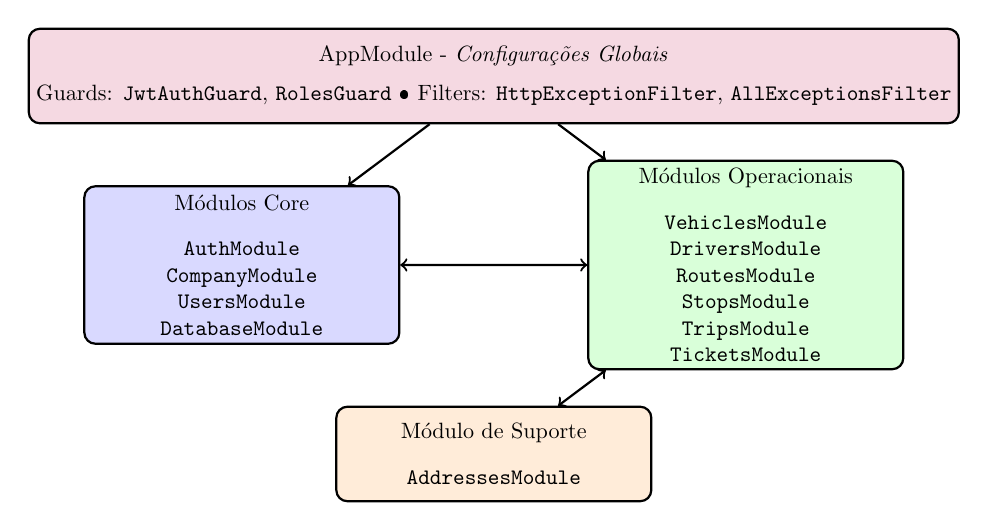
\begin{tikzpicture}[scale=0.8, every node/.style={transform shape}]
    % Módulos Core
    \node[draw, rounded corners, thick, fill=blue!15, minimum width=5cm, minimum height=2.5cm, align=center] (core) at (0,3) {
      \text{Módulos Core}\\[0.3cm]
      \texttt{AuthModule}\\
      \texttt{CompanyModule}\\
      \texttt{UsersModule}\\
      \texttt{DatabaseModule}
    };

    % Módulos Operacionais
    \node[draw, rounded corners, thick, fill=green!15, minimum width=5cm, minimum height=3cm, align=center] (operational) at (8,3) {
      \text{Módulos Operacionais}\\[0.3cm]
      \texttt{VehiclesModule}\\
      \texttt{DriversModule}\\
      \texttt{RoutesModule}\\
      \texttt{StopsModule}\\
      \texttt{TripsModule}\\
      \texttt{TicketsModule}
    };

    % Módulos de Suporte
    \node[draw, rounded corners, thick, fill=orange!15, minimum width=5cm, minimum height=1.5cm, align=center] (support) at (4,0) {
      \text{Módulo de Suporte}\\[0.3cm]
      \texttt{AddressesModule}
    };

    % AppModule
    \node[draw, rounded corners, thick, fill=purple!15, minimum width=10cm, minimum height=1.5cm, align=center] (app) at (4,6) {
      \text{AppModule} - \textit{Configurações Globais}\\[0.2cm]
      Guards: \texttt{JwtAuthGuard}, \texttt{RolesGuard} • Filters: \texttt{HttpExceptionFilter}, \texttt{AllExceptionsFilter}
    };

    % Setas
    \draw[->, thick] (app) -- (core);
    \draw[->, thick] (app) -- (operational);
    \draw[<->, thick] (core) -- (operational);
    \draw[<->, thick] (support) -- (operational);
  \end{tikzpicture}
  \caption{Organização modular do backend ViaBus.}
  \label{fig:backend-modules}
\end{figure}

A organização modular agrupa os componentes por responsabilidade funcional. Os \text{Módulos Core} gerenciam autenticação, usuários, empresas e configuração de banco de dados. Os \text{Módulos Operacionais} implementam as regras de negócio específicas do domínio de transporte. O \text{Módulo de Suporte} fornece funcionalidades auxiliares como geocodificação. O \texttt{AppModule} centraliza as configurações globais de segurança e tratamento de erros, aplicadas a todos os módulos.

\subsection{Pipeline de Processamento}

Cada requisição HTTP passa por um pipeline estruturado de middleware, guards, interceptors e filters, garantindo segurança e consistência.

\begin{figure}[H]
  \centering
  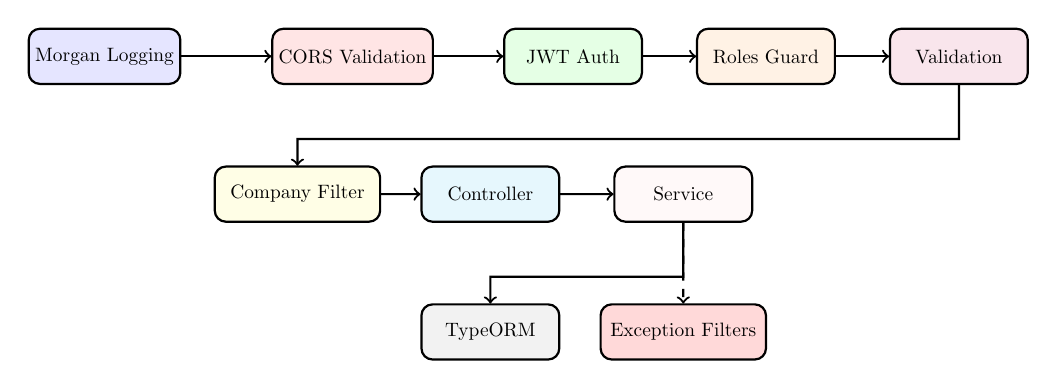
\begin{tikzpicture}[scale=0.7, every node/.style={transform shape}]
    % Pipeline stages
    \node[draw, rounded corners, thick, fill=blue!10, minimum width=2.5cm, minimum height=1cm] (morgan) at (0,0) {\text{Morgan Logging}};
    \node[draw, rounded corners, thick, fill=red!10, minimum width=2.5cm, minimum height=1cm] (cors) at (4.5,0) {\text{CORS Validation}};
    \node[draw, rounded corners, thick, fill=green!10, minimum width=2.5cm, minimum height=1cm] (jwt) at (8.5,0) {\text{JWT Auth}};
    \node[draw, rounded corners, thick, fill=orange!10, minimum width=2.5cm, minimum height=1cm] (roles) at (12,0) {\text{Roles Guard}};
    \node[draw, rounded corners, thick, fill=purple!10, minimum width=2.5cm, minimum height=1cm] (validation) at (15.5,0) {\text{Validation}};

    \node[draw, rounded corners, thick, fill=yellow!10, minimum width=3cm, minimum height=1cm] (interceptor) at (3.5,-2.5) {\text{Company Filter}};
    \node[draw, rounded corners, thick, fill=cyan!10, minimum width=2.5cm, minimum height=1cm] (controller) at (7,-2.5) {\text{Controller}};
    \node[draw, rounded corners, thick, fill=pink!10, minimum width=2.5cm, minimum height=1cm] (service) at (10.5,-2.5) {\text{Service}};

    \node[draw, rounded corners, thick, fill=gray!10, minimum width=2.5cm, minimum height=1cm] (typeorm) at (7,-5) {\text{TypeORM}};
    \node[draw, rounded corners, thick, fill=red!15, minimum width=3cm, minimum height=1cm] (filters) at (10.5,-5) {\text{Exception Filters}};

    % Arrows
    \draw[->, thick] (morgan) -- (cors);
    \draw[->, thick] (cors) -- (jwt);
    \draw[->, thick] (jwt) -- (roles);
    \draw[->, thick] (roles) -- (validation);
    \draw[->, thick] (validation) -- ++(0,-1.5) -| (interceptor);
    \draw[->, thick] (interceptor) -- (controller);
    \draw[->, thick] (controller) -- (service);
    \draw[->, thick] (service) -- ++(0,-1.5) -| (typeorm);
    \draw[->, thick, dashed] (service) -- (filters);
  \end{tikzpicture}
  \caption{Pipeline de processamento de requisições.}
  \label{fig:request-pipeline}
\end{figure}

O pipeline garante que cada requisição passe por validações sequenciais obrigatórias. Inicialmente, o \text{Morgan} registra logs e o \text{CORS} valida origens permitidas. A autenticação via \text{JwtAuthGuard} verifica tokens válidos, seguida da autorização por \text{RolesGuard} que confirma permissões do usuário. O \text{ValidationPipe} valida DTOs de entrada. O \text{CompanyFilterInterceptor} injeta o contexto multiempresa antes do processamento pelo \text{Controller} e \text{Service}. Finalmente, o \text{TypeORM} persiste dados e os \text{Exception Filters} tratam erros de forma padronizada.

\subsection{Fluxo de Autenticação}

O sistema utiliza autenticação baseada em JWT com suporte a multi-tenancy. A \autoref{fig:auth-sequence} detalha o processo completo.

\begin{figure}[H]
  \centering
  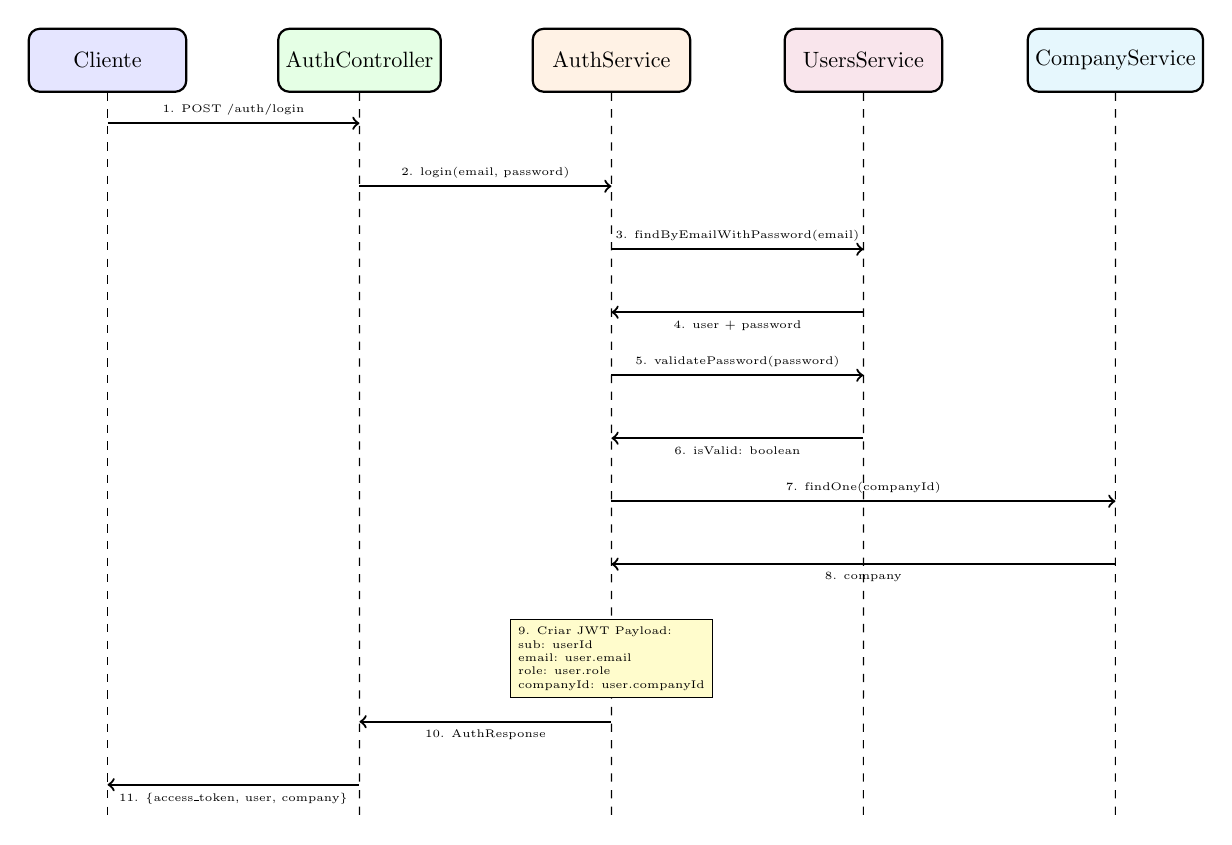
\begin{tikzpicture}[scale=0.8, every node/.style={transform shape}]
    % Participantes
    \node[draw, rounded corners, thick, fill=blue!10, minimum width=2.5cm, minimum height=1cm] (client) at (0,11) {\text{Cliente}};
    \node[draw, rounded corners, thick, fill=green!10, minimum width=2.5cm, minimum height=1cm] (auth) at (4,11) {\text{AuthController}};
    \node[draw, rounded corners, thick, fill=orange!10, minimum width=2.5cm, minimum height=1cm] (service) at (8,11) {\text{AuthService}};
    \node[draw, rounded corners, thick, fill=purple!10, minimum width=2.5cm, minimum height=1cm] (users) at (12,11) {\text{UsersService}};
    \node[draw, rounded corners, thick, fill=cyan!10, minimum width=2.5cm, minimum height=1cm] (company) at (16,11) {\text{CompanyService}};

    % Linhas de vida
    \draw[dashed] (client) -- (0,-1);
    \draw[dashed] (auth) -- (4,-1);
    \draw[dashed] (service) -- (8,-1);
    \draw[dashed] (users) -- (12,-1);
    \draw[dashed] (company) -- (16,-1);

    % Mensagens
    \draw[->, thick] (0,10) -- node[above, font=\tiny]{1. POST /auth/login} (4,10);
    \draw[->, thick] (4,9) -- node[above, font=\tiny]{2. login(email, password)} (8,9);
    \draw[->, thick] (8,8) -- node[above, font=\tiny]{3. findByEmailWithPassword(email)} (12,8);
    \draw[<-, thick] (8,7) -- node[below, font=\tiny]{4. user + password} (12,7);
    \draw[->, thick] (8,6) -- node[above, font=\tiny]{5. validatePassword(password)} (12,6);
    \draw[<-, thick] (8,5) -- node[below, font=\tiny]{6. isValid: boolean} (12,5);
    \draw[->, thick] (8,4) -- node[above, font=\tiny]{7. findOne(companyId)} (16,4);
    \draw[<-, thick] (8,3) -- node[below, font=\tiny]{8. company} (16,3);

    % Processamento interno
    \node[draw, fill=yellow!20, align=left, font=\tiny] at (8,1.5) {9. Criar JWT Payload:\\sub: userId\\email: user.email\\role: user.role\\companyId: user.companyId};

    \draw[<-, thick] (4,0.5) -- node[below, font=\tiny]{10. AuthResponse} (8,0.5);
    \draw[<-, thick] (0,-0.5) -- node[below, font=\tiny]{11. \{access\_token, user, company\}} (4,-0.5);
  \end{tikzpicture}
  \caption{Diagrama de sequência - fluxo de autenticação.}
  \label{fig:auth-sequence}
\end{figure}

O fluxo de autenticação implementa um processo seguro e eficiente em 11 etapas. O cliente envia credenciais via POST para o \texttt{AuthController}, que delega ao \texttt{AuthService} a validação. O \texttt{UsersService} busca o usuário por email (incluindo senha hash), valida a senha fornecida e retorna o resultado. Confirmada a autenticação, o \texttt{AuthService} consulta os dados da empresa via \texttt{CompanyService} e cria o payload JWT contendo informações do usuário e contexto empresarial. A resposta final inclui o token de acesso, dados do usuário e informações da empresa, permitindo que o frontend mantenha o contexto de sessão multiempresa.

\subsection{Arquitetura Multi-tenant}

O sistema implementa isolamento de dados por empresa através de uma arquitetura multi-tenant baseada em filtros automáticos. A solução utiliza três componentes principais que trabalham em conjunto para garantir separação completa entre inquilinos:

\begin{itemize}
  \item \text{BaseCompanyService<T>}: Classe abstrata que implementa operações CRUD com filtro automático por \texttt{companyId}
  \item \text{CompanyFilterInterceptor}: Interceptor que extrai o \texttt{companyId} do token JWT e o injeta no contexto da requisição
  \item \text{@CurrentUser}: Decorator que facilita o acesso aos dados do usuário autenticado
\end{itemize}

A implementação garante que todas as operações de banco de dados incluam automaticamente a cláusula \texttt{WHERE companyId = ?}, eliminando a possibilidade de vazamento de dados entre empresas. O padrão é aplicado consistentemente em todos os módulos operacionais (usuários, motoristas, veículos, rotas, paradas, viagens e passagens).

\begin{figure}[H]
  \centering
  \begin{tikzpicture}[
      % Estilos para os nós do diagrama
      tenant/.style={
          rectangle,
          rounded corners,
          draw,
          thick,
          fill=blue!10,
          minimum height=1cm,
          font=\small
        },
      application/.style={
          rectangle,
          rounded corners,
          draw,
          thick,
          fill=purple!20,
          minimum width=8cm,
          minimum height=1.5cm,
          font=\bfseries
        },
      database/.style={
          cylinder,
          shape border rotate=90,
          draw,
          thick,
          fill=gray!20,
          minimum height=4cm, %<-- Aumentado
          minimum width=4.5cm,    %<-- Aumentado
          aspect=0.25
        },
      label/.style={
          font=\footnotesize\itshape,
          text=gray!80!black
        }
    ]

    % --- Nível 1: Requisições dos Clientes (Tenants) ---
    \node[tenant] (tenantA) at (-4, 5) {Empresa A};
    \node[tenant] (tenantB) at (0, 5)  {Empresa B};
    \node[tenant] (tenantC) at (4, 5)  {Empresa C};

    % --- Nível 2: Aplicação Única ---
    \node[application] (app) at (0, 2.5) {Aplicação ViaBus (Instância Única)};

    % --- Nível 3: Camada de Identificação ---
    \node[trapezium, draw, thick, fill=orange!20, shape border rotate=180, minimum width=4cm] (jwt) at (0, 0.5) {
      \small\bfseries Filtro de Autenticação (JWT)
    };
    \node[label, below=0.1 of jwt] {\textit{companyId} extraído do token};

    % --- Nível 4: Banco de Dados com Dados Isolados ---
    % Movido para baixo para acomodar o novo tamanho
    \node[database, label={[label distance=-1.5cm]90:\textbf{Banco de Dados}}] (db) at (0, -3) {};

    % Partições lógicas dentro do banco de dados (ajustadas)
    \node[font=\tiny, fill=blue!25, draw, rounded corners] at (-1, -3.2) {Empresa A};
    \node[font=\tiny, fill=green!25, draw, rounded corners] at (0, -3.8) {Empresa B};
    \node[font=\tiny, fill=orange!25, draw, rounded corners] at (1, -3.2) {Empresa C};
    % Label "Dados Isolados" movido para baixo
    \node[font=\small\bfseries] at (0, -4.5) {DB - Dados Isolados};

    % --- Setas de Fluxo (ajustadas para as novas posições) ---
    \draw[-{Stealth[length=3mm]}, thick] (tenantA.south) -- (app.north);
    \draw[-{Stealth[length=3mm]}, thick] (tenantB.south) -- (app.north);
    \draw[-{Stealth[length=3mm]}, thick] (tenantC.south) -- (app.north);

    \draw[-{Stealth[length=3mm]}, thick] (app.south) -- (jwt.north);

    \draw[-{Stealth[length=3mm]}, thick, blue!50!black] (jwt.south) to[out=-135, in=90] (-1, -2.8);
    \draw[-{Stealth[length=3mm]}, thick, green!50!black] (jwt.south) to[out=-90, in=90] (0, -3.4);
    \draw[-{Stealth[length=3mm]}, thick, orange!50!black] (jwt.south) to[out=-45, in=90] (1, -2.8);

  \end{tikzpicture}
  \caption{Arquitetura multi-tenant: uma única aplicação com dados logicamente isolados por empresa no banco de dados.}
  \label{fig:multi-tenant-melhorada}
\end{figure}

\section{Arquitetura do Frontend}

O frontend implementa uma arquitetura moderna baseada em Next.js~15 (React~19) com seu \textit{App Router}, utilizando TypeScript para garantir uma tipagem estática completa. A aplicação foi estruturada seguindo padrões de arquitetura limpa e uma organização orientada a domínios de negócio, visando a manutenibilidade e a escalabilidade da interface.

\subsection{Stack Tecnológico e Organização}

Para garantir performance, uma boa experiência de usuário e manutenibilidade, o frontend utiliza um conjunto integrado de tecnologias. A base da aplicação é o \text{Next.js~15}, que, junto ao \text{React~19}, oferece uma plataforma sólida para a renderização da interface. A construção da UI segue um \textit{design system} customizado, empregando componentes primitivos do \text{Radix UI} para assegurar a acessibilidade e o \text{Tailwind CSS} para uma estilização \textit{utility-first} ágil e consistente. A gestão de formulários é responsabilidade do \text{React Hook Form} combinado com o \text{Zod} para validação tipada de dados. A autenticação é gerenciada pelo \text{NextAuth v4}, enquanto as funcionalidades geográficas são implementadas com \text{Leaflet}. O estado global da aplicação, por sua vez, é controlado de forma eficiente pela \text{Context API} nativa do \text{React}.

\subsection{Arquitetura de Roteamento}

A aplicação utiliza o \textit{App Router} do Next.js~15, que permite um roteamento dinâmico e baseado em arquivos. A estrutura de rotas foi projetada para suportar a natureza multiempresa do sistema, seguindo o padrão \texttt{/dashboard/[company]/recurso}. Essa abordagem garante o isolamento dos dados no nível da URL, onde cada empresa acessa seus próprios recursos, como \texttt{/motoristas} ou \texttt{/rotas}, dentro de seu próprio escopo. O sistema diferencia entre páginas públicas, como \texttt{/login} e \texttt{/criar-empresa}, e as rotas privadas do \textit{dashboard}. A proteção de rotas é garantida por um componente de ordem superior (\textit{wrapper}) chamado \texttt{ProtectedPage}, que valida a autenticação e as permissões do usuário antes de renderizar a página solicitada.

\subsection{Gerenciamento de Estado e Contextos}

O gerenciamento do estado global da aplicação é implementado através de uma hierarquia de \textit{Contextos} React. Essa abordagem permite um compartilhamento de dados eficiente e desacoplado entre os componentes. No topo da hierarquia, o \texttt{SessionProvider} gerencia a sessão do NextAuth e os tokens JWT. Abaixo dele, o \texttt{ThemeProvider} controla o tema visual da aplicação (claro/escuro). Em seguida, o \texttt{AuthProvider} expõe os dados do usuário autenticado e da empresa associada. O \texttt{CompanyProvider} mantém o estado específico da empresa que está sendo visualizada no \textit{dashboard}, enquanto o \texttt{SidebarProvider}, na camada mais interna, gerencia estados de UI, como a visibilidade do menu lateral.

\subsection{Sistema de Autenticação e Comunicação}

A comunicação com o backend é centralizada para garantir consistência e segurança. A autenticação integra o NextAuth com a API NestJS através de tokens JWT, e todas as requisições HTTP são gerenciadas por um serviço centralizado, o \texttt{api.service.ts}. Este serviço encapsula responsabilidades críticas: ele anexa automaticamente os \textit{Bearer tokens} de autenticação em todas as chamadas a rotas protegidas, trata respostas de erro de forma padronizada (redirecionando para a página de login em caso de erro 401, por exemplo), processa as respostas da API para extrair os dados e valida a sessão do usuário antes de cada requisição, otimizando a comunicação com o servidor.

\subsection{Arquitetura de Componentes}

O sistema de componentes foi projetado em camadas, seguindo uma lógica de composição que vai do mais simples ao mais complexo. Na base, estão os Primitivos de UI do Radix UI, que fornecem comportamento e acessibilidade sem estilização. Sobre eles, foi construído um Design System de componentes reutilizáveis e tipados (localizados em \texttt{components/ui/}), que definem a aparência visual da aplicação. Estes são, então, utilizados para compor os Componentes de Domínio, que são específicos de cada funcionalidade, como formulários de cadastro ou tabelas de dados. Por fim, as Páginas são montadas através da composição desses componentes, organizadas dentro de Layouts reutilizáveis que fornecem a estrutura de navegação e os provedores de contexto necessários.


\subsection{Tipagem e Validação}

O TypeScript é utilizado de forma extensiva para garantir a integridade dos dados em toda a aplicação. Um diretório central de tipos (\textit{Types Directory}) contém as definições para cada entidade de negócio (\texttt{User}, \texttt{Company}, etc.), servindo como uma fonte única da verdade para a estrutura de dados. Essa tipagem se estende às respostas da API, garantindo que os dados recebidos do backend correspondam ao esperado. No lado do cliente, a validação de formulários é realizada com \textit{Schemas} Zod, que asseguram a consistência dos dados antes do envio. Essa abordagem cria uma arquitetura com tipagem estática de ponta a ponta (\textit{end-to-end}), desde o banco de dados até a interface do usuário.

\begin{figure}[htbp]
  \centering
  \begin{tikzpicture}[
      scale=0.8,
      every node/.style={transform shape},
      node distance=1.5cm,
      layer/.style={
          rectangle,
          draw,
          thick,
          rounded corners,
          fill=#1,
          minimum width=9cm,
          minimum height=1.8cm,
          align=center,
          text width=8.5cm,
          font=\bfseries\small
        },
      actor/.style={
          font=\bfseries\small,
          rectangle,
          draw,
          fill=gray!15,
          rounded corners,
          minimum width=2cm
        },
      arrow/.style={-Stealth, thick}
    ]

    % --- Nível 1: Atores Externos ---
    \node[actor] (user) at (-7, 6.5) {Usuário};
    \node[actor] (backend) at (7, -0.5) {Backend API};

    % --- Camadas da Aplicação Frontend ---
    \node[layer=blue!15] (view) at (0, 4.5) {
      Camada de Visualização \\
      \normalfont{\small (\textit{App Router}, Páginas, Layouts, Componentes de UI e Domínio)}
    };

    \node[layer=green!15] (logic) at (0, 2) {
      Camada de Lógica e Estado \\
      \normalfont{\small (Contextos, Hooks, Validação Zod, React Hook Form)}
    };

    \node[layer=red!15] (data) at (0, -0.5) {
      Camada de Acesso a Dados \\
      \normalfont{\small (\texttt{api.service.ts}, NextAuth - Gerenciamento de Tokens)}
    };

    % --- Fluxo de Dados ---
    % Usuário -> View
    \draw[arrow] (user.east) to[out=0, in=180] node[pos=0.5, above, font=\tiny]{Interage com UI / Navega} (view.west);

    % View <-> Lógica (bidirecional para interação e estado)
    \draw[arrow] (view.south) -- node[left, font=\tiny]{1. Dispara Ações / Solicita Dados} (logic.north);
    \draw[arrow] (logic.north) -- node[right, font=\tiny]{4. Atualiza Estado / UI} (view.south);

    % Lógica <-> Dados (bidirecional para requisição e resposta)
    \draw[arrow] (logic.south) -- node[left, font=\tiny]{2. Chama Serviço API} (data.north);
    \draw[arrow] (data.north) -- node[right, font=\tiny]{3. Retorna Resposta API} (logic.south);

    % Dados <-> Backend
    \draw[arrow] (data.east) -- (backend.west);

  \end{tikzpicture}
  \caption{Arquitetura em camadas do frontend e fluxo de dados principal.}
  \label{fig:arquitetura-frontend-simplificada}
\end{figure}

\section{Estratégia de Implantação}

A implantação do sistema ViaBus foi planejada em uma arquitetura de nuvem, utilizando um conjunto de serviços da Google Cloud Platform (GCP) para automação e escalabilidade. A estratégia adotada consistiu em quatro etapas principais: conteinerização da aplicação, implantação dos serviços em ambiente \textit{serverless}, gerenciamento do banco de dados e automação da entrega (CI/CD).

Para garantir a portabilidade entre os ambientes, a aplicação foi conteinerizada com Docker. Foram criados arquivos \texttt{Dockerfile} específicos para o \textit{backend} (NestJS) e o \textit{frontend} (Next.js), utilizando a abordagem de \textit{multi-stage builds} para gerar imagens otimizadas e seguras. A orquestração do ambiente de desenvolvimento local foi realizada com o Docker Compose.

Os contêineres da aplicação foram implantados na nuvem como dois serviços independentes no Google Cloud Run, uma plataforma de computação \textit{serverless}. Essa configuração permite que o \textit{frontend} e o \textit{backend} escalem de forma autônoma com base na demanda de requisições. A comunicação externa é garantida via HTTPS, com certificados TLS/SSL gerenciados automaticamente pela plataforma.

Para a persistência dos dados, foi utilizada uma instância gerenciada do PostgreSQL no serviço Google Cloud SQL. A comunicação entre a API executada no Cloud Run e o banco de dados ocorre em uma rede segura e privada, com criptografia dos dados em trânsito e em repouso. A responsabilidade por tarefas de manutenção, como backups e atualizações, é delegada ao próprio serviço da GCP.

Por fim, o ciclo de vida da aplicação foi automatizado com práticas de Integração e Entrega Contínuas (CI/CD). Foram estruturados ambientes isolados de desenvolvimento e produção na GCP. O gerenciamento de informações sensíveis, como chaves de API e credenciais de banco de dados, foi centralizado no Google Secret Manager. Um \textit{pipeline} no Google Cloud Build foi configurado para automatizar o processo de construção das imagens Docker e a implantação de novas versões no Cloud Run a cada atualização no repositório principal do Git.